%State Chart Syntax
\section{Syntax of The State Chart Language}

Abstract syntax of our state chart language:

\begin{itemize}
	\item Expression := Expression Op Expression $|$ Op Expression
	\item Var := Expression | Constant
	\item Type := Char | Int | Long | Bool | Float
	\item Identifier := [a-zA-Z$\_$]+[a-zA-Z0-9$\_$]*  
	
	\item StoreBlock := Type Identifier = Var | Type Identifier = Var StoreBlock

	\item Condition := Var Eq Var | Var Eq Condition | Condition Eq Condition
	
	\item Eq := $=$ | $\neq$ | $<$ | $\leq$ | $>$ | $\geq$	
	
	\item Transition := StoreBlock | Condition | Storeblock
	
\end{itemize}

\begin{figure}[htp]
    \centering
    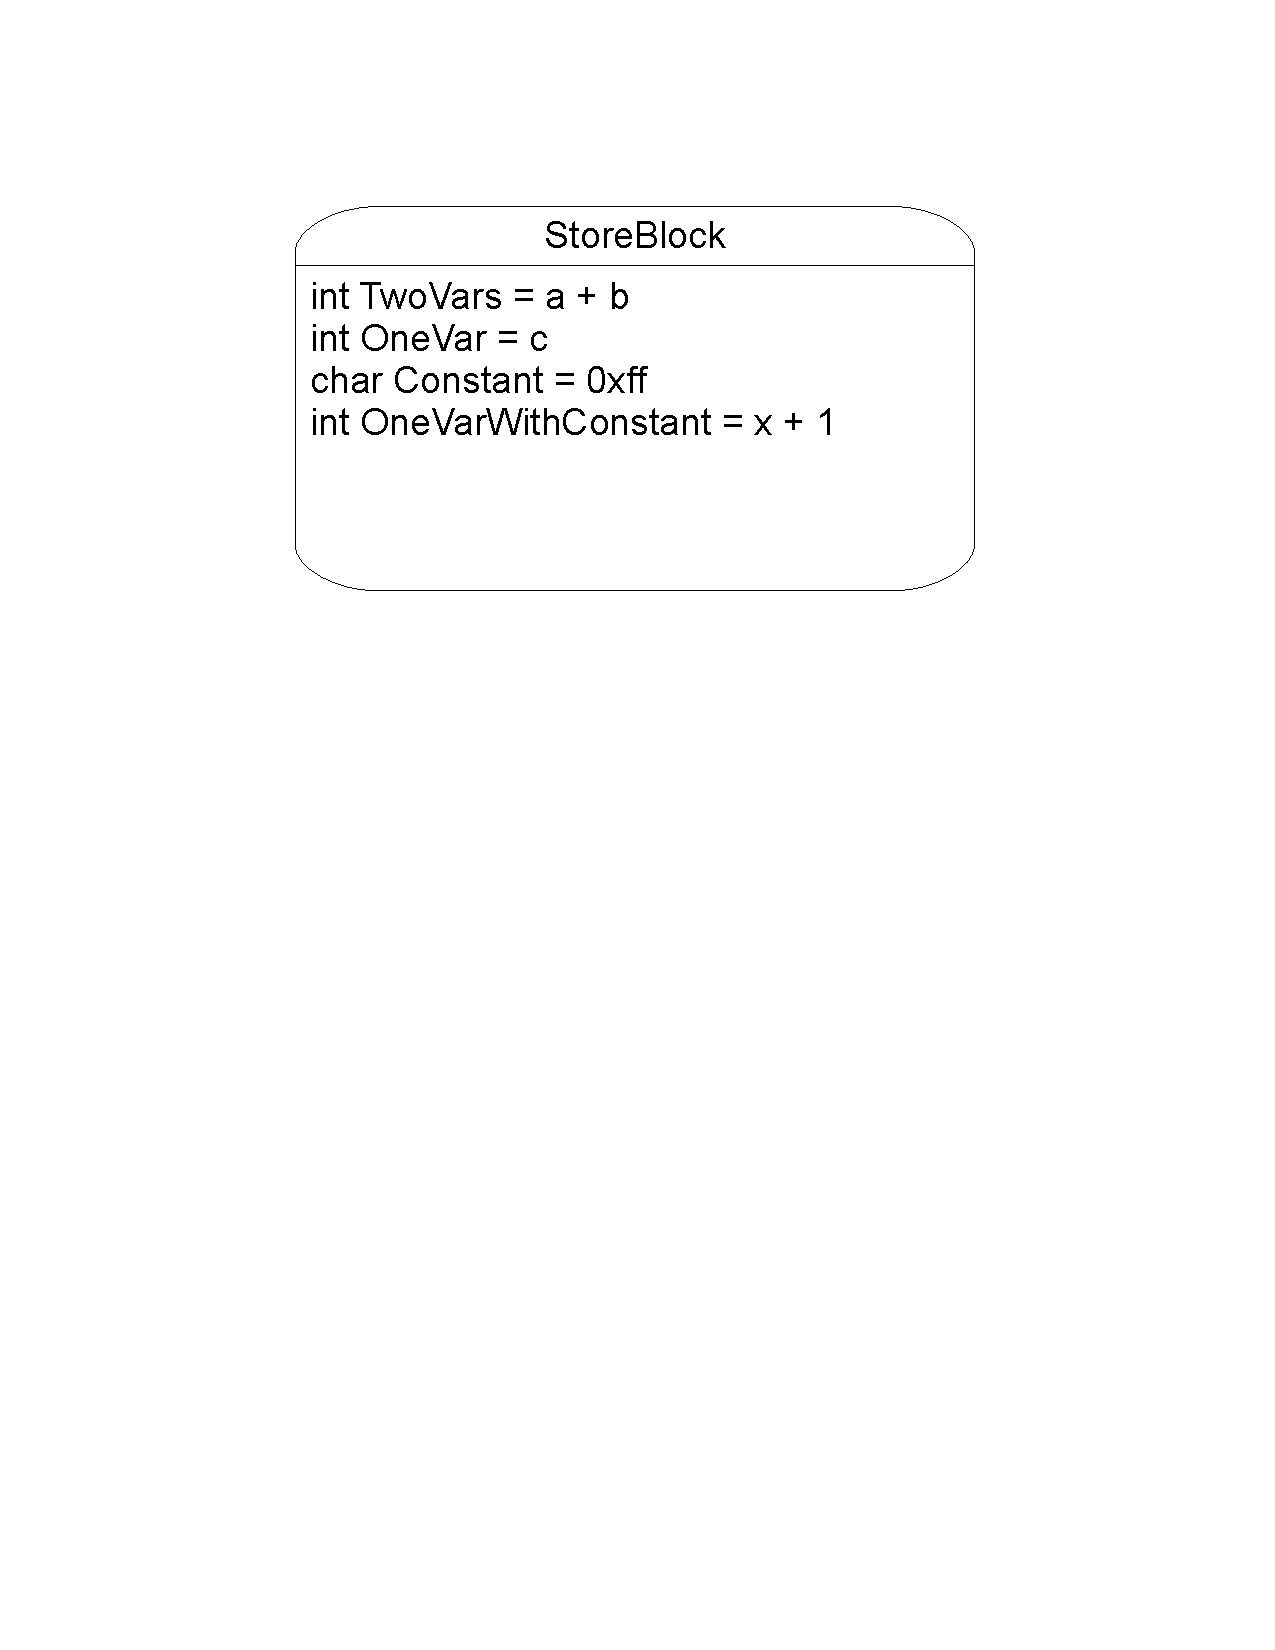
\includegraphics[trim= 20mm 170mm 20mm 10mm, clip, width=\imgmedium]{./images/state_storeblock.pdf}
    \caption{Example Of A Store Block As Implemented In PLCEdit}
    \label{fig:state_storeblock}
\end{figure}

TODO: DRAW storeblock point out identifier type var and "assignment"

TODO: Draw transitions point out coundition

